% Figure: the duality behind the algorithm for subcomplexes of the 3-sphere, shown one dimension lower.
% Requires only tikz. The dual-graph coordinates were generated by a short script (components computed, not drawn by hand).
\begin{figure}[t]
\centering
\providecommand\Description[2][]{}%
\Description{A large triangle subdivided into sixteen small triangles. A thick black hexagon surrounds one vertex and a filled triangle sits at the top corner. Blue dots and edges connect the six triangles inside the hexagon; green dots and edges connect the triangles outside, with dashed green stubs leading out to the outer face.}
\definecolor{duA}{HTML}{0072B2}%
\definecolor{duB}{HTML}{009E73}%
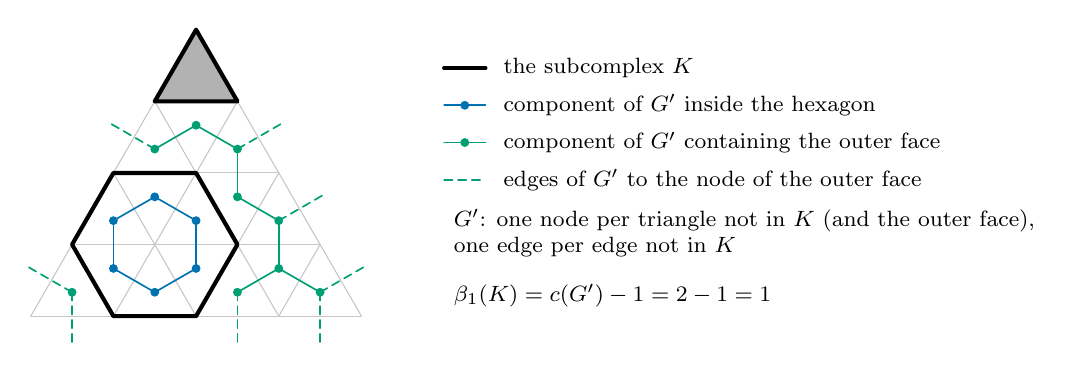
\begin{tikzpicture}[x=1.05cm,y=1.05cm,line join=round,line cap=round]
  % the triangulation T of a big triangle of side 4 (together with the outer face, a triangulated 2-sphere)
  \foreach \j in {0,...,3} {
    \pgfmathtruncatemacro{\m}{3-\j}
    \foreach \i in {0,...,\m} {
      \draw[black!22,line width=0.4pt] ({\i+0.5*\j},{0.866*\j}) -- ({\i+1+0.5*\j},{0.866*\j});
      \draw[black!22,line width=0.4pt] ({\i+0.5*\j},{0.866*\j}) -- ({\i+0.5*(\j+1)},{0.866*(\j+1)});
      \draw[black!22,line width=0.4pt] ({\i+1+0.5*\j},{0.866*\j}) -- ({\i+0.5*(\j+1)},{0.866*(\j+1)});
    }}
  % the filled triangle of K
  \fill[black!30] (1.5,2.598) -- (2.5,2.598) -- (2,3.464) -- cycle;
  % the graph G': nodes = triangles not in K, edges = edges not in K; dashed stubs lead to the outer face
\draw[duA,line width=0.6pt] (1.000,0.577) -- (1.500,0.289);
\draw[duA,line width=0.6pt] (1.000,0.577) -- (1.000,1.155);
\draw[duA,line width=0.6pt] (1.500,0.289) -- (2.000,0.577);
\draw[duA,line width=0.6pt] (2.000,0.577) -- (2.000,1.155);
\draw[duB,line width=0.6pt] (2.500,0.289) -- (3.000,0.577);
\draw[duB,line width=0.6pt] (3.000,0.577) -- (3.500,0.289);
\draw[duB,line width=0.6pt] (3.000,0.577) -- (3.000,1.155);
\draw[duA,line width=0.6pt] (1.000,1.155) -- (1.500,1.443);
\draw[duA,line width=0.6pt] (1.500,1.443) -- (2.000,1.155);
\draw[duB,line width=0.6pt] (2.500,1.443) -- (3.000,1.155);
\draw[duB,line width=0.6pt] (2.500,1.443) -- (2.500,2.021);
\draw[duB,line width=0.6pt] (1.500,2.021) -- (2.000,2.309);
\draw[duB,line width=0.6pt] (2.000,2.309) -- (2.500,2.021);
\draw[duB,line width=0.6pt,densely dashed] (0.500,0.289) -- (0.500,-0.320);
\draw[duB,line width=0.6pt,densely dashed] (0.500,0.289) -- (-0.027,0.593);
\draw[duB,line width=0.6pt,densely dashed] (2.500,0.289) -- (2.500,-0.320);
\draw[duB,line width=0.6pt,densely dashed] (3.500,0.289) -- (3.500,-0.320);
\draw[duB,line width=0.6pt,densely dashed] (3.500,0.289) -- (4.027,0.593);
\draw[duB,line width=0.6pt,densely dashed] (3.000,1.155) -- (3.527,1.459);
\draw[duB,line width=0.6pt,densely dashed] (1.500,2.021) -- (0.973,2.325);
\draw[duB,line width=0.6pt,densely dashed] (2.500,2.021) -- (3.027,2.325);
\fill[duB] (0.500,0.289) circle (1.6pt);
\fill[duA] (1.000,0.577) circle (1.6pt);
\fill[duA] (1.500,0.289) circle (1.6pt);
\fill[duA] (2.000,0.577) circle (1.6pt);
\fill[duB] (2.500,0.289) circle (1.6pt);
\fill[duB] (3.000,0.577) circle (1.6pt);
\fill[duB] (3.500,0.289) circle (1.6pt);
\fill[duA] (1.000,1.155) circle (1.6pt);
\fill[duA] (1.500,1.443) circle (1.6pt);
\fill[duA] (2.000,1.155) circle (1.6pt);
\fill[duB] (2.500,1.443) circle (1.6pt);
\fill[duB] (3.000,1.155) circle (1.6pt);
\fill[duB] (1.500,2.021) circle (1.6pt);
\fill[duB] (2.000,2.309) circle (1.6pt);
\fill[duB] (2.500,2.021) circle (1.6pt);

  % K: a hexagonal 1-cycle and a filled triangle
  \draw[black,line width=1.5pt] (2,0) -- (2.5,0.866) -- (2,1.732) -- (1,1.732) -- (0.5,0.866) -- (1,0) -- cycle;
  \draw[black,line width=1.5pt] (1.5,2.598) -- (2.5,2.598) -- (2,3.464) -- cycle;
  % legend
  \begin{scope}[shift={(5.0,3.0)},font=\footnotesize]
    \draw[black,line width=1.5pt] (0,0) -- (0.5,0); \node[anchor=west] at (0.6,0) {the subcomplex $K$};
    \draw[duA,line width=0.6pt] (0,-0.45) -- (0.5,-0.45); \fill[duA] (0.25,-0.45) circle (1.6pt);
    \node[anchor=west] at (0.6,-0.45) {component of $G'$ inside the hexagon};
    \draw[duB,line width=0.6pt] (0,-0.9) -- (0.5,-0.9); \fill[duB] (0.25,-0.9) circle (1.6pt);
    \node[anchor=west] at (0.6,-0.9) {component of $G'$ containing the outer face};
    \draw[duB,line width=0.6pt,densely dashed] (0,-1.35) -- (0.5,-1.35);
    \node[anchor=west] at (0.6,-1.35) {edges of $G'$ to the node of the outer face};
    \node[anchor=west,align=left] at (0,-2.0) {$G'$: one node per triangle not in $K$ (and the outer face),\\one edge per edge not in $K$};
    \node[anchor=west] at (0,-2.75) {$\beta_1(K)=c(G')-1=2-1=1$};
  \end{scope}
\end{tikzpicture}
\caption{The duality behind Theorem~\ref{thm:s3}, one dimension lower.
For a proper subcomplex $K$ of a triangulated $2$-sphere, of which only a triangulated disk is drawn (the triangles outside the disk are not in~$K$ and are merged into one node, the outer face), Alexander duality gives $\beta_1(K)=c-1$, where $c$ is the number of components of the complement of~$K$, and these components are the components of the graph~$G'$ whose nodes are the triangles not in~$K$ (and the outer face) and whose edges are the edges not in~$K$, as in the proof of Lemma~\ref{lem:dual}.
A simplex update changes $G'$ by $O(1)$ nodes or edges, so dynamic connectivity maintains~$\beta_1(K)$.
For a triangulated $3$-sphere, the same argument applies to $\beta_2$, with tetrahedra as nodes and triangles as edges.}
\label{fig:duality}
\end{figure}
